%------------------------------------------------------------------------------
% Template file for the submission of papers to IUCr journals in LaTeX2e
% using the iucr document class
% Copyright 1999-2013 International Union of Crystallography
% Version 1.6 (28 March 2013)
%------------------------------------------------------------------------------

\documentclass{iucr}              % DO NOT DELETE THIS LINE
\usepackage{bm}
% \usepackage{graphicx}
% \usepackage{tabularx}
% \usepackage{subfigure}
% \usepackage{afterpage}
% \usepackage{sansmath}
\usepackage{mathtools}
% \usepackage{parskip}
% \usepackage{tikz}
% \usepackage{tikzorbital}
% \usepackage{setspace}
% \usepackage{xcolor}
% \usepackage{amssymb}
% \usepackage{bm}
\usepackage{amsmath}
% \usepackage{fancyhdr}
% \usepackage{rotating}
% \usepackage{siunitx}
\usepackage[hyphens,spaces,obeyspaces]{url}
\usepackage{color}
\usepackage{siunitx}
\usepackage[hyphens,spaces,obeyspaces]{url}
\usepackage{color}
\usepackage{cprotect}
\usepackage{textgreek}
\usepackage[normalem]{ulem}

\newcommand{\todo}[1]{{\color{red}[TODO: "#1'']}}
\newcommand{\inblue}[1]{{\color{blue}#1}}
\newcommand{\inred}[1]{{\color{red}#1}}
\newcommand{\ingreen}[1]{{\color{green}#1}}

     %-------------------------------------------------------------------------
     % Infobrmation about journal to which submitted
     %-------------------------------------------------------------------------
     \journalcode{A}              % Indicate the journal to which submitted
                                  %   A - Acta Crystallographica Section A
                                  %   B - Acta Crystallographica Section B
                                  %   C - Acta Crystallographica Section C
                                  %   D - Acta Crystallographica Section D
                                  %   E - Acta Crystallographica Section E
                                  %   F - Acta Crystallographica Section F
                                  %   J - Journal of Applied Crystallography
                                  %   M - IUCrJ
                                  %   S - Journal of Synchrotron Radiation

\begin{document}                  % DO NOT DELETE THIS LINE

     %-------------------------------------------------------------------------
     % The introductory (header) part of the paper
     %-------------------------------------------------------------------------

     % The title of the paper. Use \shorttitle to indicate an abbreviated title
     % for use in running heads (you will need to uncomment it).

\title{X-ray focusing by bent crystals: focal positions as predicted by the Crystal lens equation and the Dynamical Diffraction Theory}
% * <msanchezdelrio@gmail.com> 2018-09-25T09:38:50.716Z:
%
% ^.
%\shorttitle{Short Title}

     % Authors' names and addresses. Use \cauthor for the main (contact) author.
     % Use \author for all other authors. Use \aff for authors' affiliations.
     % Use lower-case letters in square brackets to link authors to their
     % affiliations; if there is only one affiliation address, remove the [a].

\cauthor[a]{Jean-Pierre}{Guigay}{guigay@esrf.eu}{address if different from \aff}
\author[a]{Manuel}{Sanchez del Rio}


\aff[a]{European Synchrotron Radiation Facility, 71 Avenue des Martyrs F-38000 Grenoble \country{France}}
\aff[b]{XXX \country{Finland}}


     % Use \shortauthor to indicate an abbreviated author list for use in
     % running heads (you will need to uncomment it).

%\shortauthor{Soape, Author and Doe}

     % Use \vita if required to give biographical details (for authors of
     % invited review papers only). Uncomment it.

%\vita{Author's biography}

     % Keywords (required for Journal of Synchrotron Radiation only)
     % Use the \keyword macro for each word or phrase, e.g. 
     % \keyword{X-ray diffraction}\keyword{muscle}

%\keyword{keyword}

     % PDB and NDB reference codes for structures referenced in the article and
     % deposited with the Protein Data Bank and Nucleic Acids Database (Acta
     % Crystallographica Section D). Repeat for each separate structure e.g
     % \PDBref[dethiobiotin synthetase]{1byi} \NDBref[d(G$_4$CGC$_4$)]{ad0002}

%\PDBref[optional name]{refcode}
%\NDBref[optional name]{refcode}

\maketitle                        % DO NOT DELETE THIS LINE

\begin{synopsis}
The location of the focal waist when x-ray radiation encounters a bent crystals is addressed from a theoretical point of view with numerical validation.
\end{synopsis}

\begin{abstract}
The location of the focal waist when x-ray radiation encounters a bent crystals is addressed from a theoretical point of view with numerical validation.
\end{abstract}


     %-------------------------------------------------------------------------
     % The main body of the paper
     %-------------------------------------------------------------------------
     % Now enter the text of the document in multiple \section's, \subsection's
     % and \subsubsection's as required.

\section{Introduction}

The use of curved crystals to diffract and focus X-rays was a natural extension of the principles used in mirror and grating technology for radiation of longer wavelength. Some fundamental concepts exported to crystal optics, like the Rowland circle, date back to the XIX century \cite{rowland1882}.

The fundamental mounting types using bent crystals focusing were proposed in the early 1930’s. Systems exploiting meridional focusing are: i) Johann spectrometer \cite{Johann1931}, that uses a cylindrically bent crystal,  ii) Johansson spectrometer \cite{Johansson1933} that uses a ground and cylindrically bent crystal, iii) the Cauchois spectrometer \cite{cauchois1933} exploiting a Laue crystal. The von Hamos spectrometer \cite{V.Hamos1933} apply sagittal focusing in the plane perpendicular to the diffraction plane.

With the advent of Synchrotron Radiation, the concepts of geometrical focusing were applied to design instruments such as polychromators for energy-dispersive Extended X-ray Absorption Fine Structure (EXAFS) \cite{Tolentino:ms0206}, monochromators with sagittal focusing for bending magnet beamlines \inred{(REF)} or bent Laue crystals for high energy beamlines, in which the curvature is used for focusing or collimating the beam or just to enlarge the energy bandwidth and improve the luminosity. The concepts of crystal bandwidth and aberrations came into play to better profit of the good characteristics of synchrotron beams, particularly the good collimation and small source size. For beamline monochromators  most systems work out of the Rowland conditions, whereas crystal analysers for applications such as inelastic scattering studies apply the Rowland setting.

The geometrical theory of image formation for mirrors working in grazing incidence gives a first idea of the image formed by reflection of meridional rays at a spherical reflector \cite{KB1948}. The Gaussian mirror equation (mirror or lens equation), relates the object distance $p$ and the image distance $q$ to the focal length $f$, $p^{-1}+q^{-1}=f^{-1}$, with $f=R \sin\theta$, where $R$ is the mirror curvature radius and $\theta$ the grazing incidence angle. However, this mirror or lens equation has limited applications when using crystals, as it can be applied only for symmetric Bragg reflections. The conservation of the tangential component of the wavevector on the crystal surface leads to more general equations in Bragg or Laue geometries, resembling the focusing equations for reflection or transmission gratings.

A ``Crystal lens equation" (CLE) was indeed formulated by \cite{CK} for the focusing properties of a cylindrically bent crystal plate in Bragg diffraction of monochromatic X-rays or neutrons, in Laue (transmission) or Bragg (reflection) geometry, the crystal being bent around an axis perpendicular to the diffraction plane (meridional focusing). This CLE is based on a purely geometric approach in which the multiple scattering processes in the crystal (dynamical effects) are not taken into account. We have realised that, because of  algebra errors, the CLE form given in the above cited article is not correct in Laue geometry; therefore, the calculations are repeated and a revised form of the CLE is presented in Section~\ref{sec:CLE}.

The CLE utility is strongly restricted in the case of Laue geometry because it is only applicable to a crystal plate of vanishing thickness, therefore of vanishing reflectivity. Moreover, it does not give account of a dynamical focusing phenomenon first  predicted in the case of flat crystals by \cite{AfanasevKohn1977} and confirmed experimentally by references \cite{Aristov1978} and \cite{Aristov1980} . We present. in section~\ref{sec:CLE}, a simple and general description of the focusing effect in the case of a flat crystal plate of finite thickness and we use it to obtain an improved form of the CLE for a bent crystal (presently, only in the case of symmetric reflection). 
\inblue{COMPLETE: We also verify that the dynamical formulation used in \cite{GuigayFerrero2016} agrees with the CLE in the limit of vanishing crystal thickness, as expected. In discussing the case of symmetrical geometry, we show the important role played by the ``length of dynamical focusing",  which depends on the parameters of the unbent crystal. The elements of the dynamical theory used in the present paper can be found in the textbook of \cite{authierbook}.

The application of the lens equation in symmetrical Bragg geometry is discussed in sect.4, with comparison to recent numerical simulations \cite{Honkanen2018}) which are based on a finite element method to take the propagation in the crystal into account.

The CLE is in general different from the well known conditions of polychromatic focusing. Particular cases of coincidence of these two focusing conditions are considered.   
}

\section{Lens equation revisited}
\label{sec:CLE}

A lens equation was derived by \cite{CK} in the case of a monochromatic X-ray or neutron wave which is Bragg-reflected by a cylindrically bent crystal plate. We repeat this derivation here fixing some problem found in their derivation. 

Consider a monochromatic X-ray or neutron beam emitted by a point-source $S$. The origin of coordinates is chosen at the point $O$ of the crystal surface in which the incident ray $\vec{SO}$, of wave-vector  ${\vec k_0}$, is in exact Bragg  position. The diffracted ray has a wave-vector $\vec k_h$ given by the Laue equation $\vec k_h = \vec k_0 + \vec h$, where $\vec h$ is the \inblue{reciprocal lattice vector}. This is valid for both transmission geometry (Laue) or reflection geometry (Bragg). We use oriented angles $\varphi_0 = (\vec n, \vec k_0)$ and $\varphi_h = (\vec n, \vec k_h)$, where $\vec n$ is the inward normal to the crystal surface. $\varphi_0$ is positive, without loss of generality \inred{but it can be in any quadrant???}. Defining $\vec k_0^{sym}$ the $\vec k_0$ vector for the symmetric (Bragg or Laue) case, it allows to define the asymmetry angle as the departure of $\vec k_0$ from its position for symmetrical case $\alpha = (\vec k_0^{sym}, \vec k_0)$ \todo{WOULD BE BETTER TO DEFINE IT AS the departure of $\vec H$ from its position for symmetrical case $\alpha = (\vec H^{sym}, \vec H)$}. Let be $\theta_B$ the \inred{unsigned} Bragg angle. With these definitions $\theta_B=(\varphi_0-\varphi_h)/2$ and $2\alpha=\varphi_0+\varphi_h$ for the Laue case;  $\theta_B=(\varphi_h-\varphi_0)/2$  and  $2\alpha+\pi=\varphi_0+\varphi_h$for the  Bragg case. 

The source distance $L_0$ is set as positive if the source is on the incidence side of the crystal (real source) or negative if the source is on the other side (virtual source) (see Fig.~\ref{FIG_LENS1})
When moving the point of incidence over a small distance $s$ along the curved crystal surface, $\vec{k_{0,h}}$ are changed in direction, with rotating angles $\epsilon_{0,h} = (\vec k_{0,h},\vec k'_{0,h})$, and $\varphi_{0,h}$ are changed into $\varphi'_{0,h}=\varphi_{0,h}+\Delta \varphi_{0,h}$.

The projection of  ${\vec k'_h}$ and $(\vec k'_0 + \vec h')$ on the crystal surface are equal \inred {as a result of conservation of the parallel component of the wave-vector}. The projection of $\vec h'$ \inred{onto the crystal surface} is constant\inred{ because the asymmetry angle does not change ($\vec H$ and $\vec n$ are rigidly attached when moving}. This implies that $(\sin \varphi_h - \sin \varphi_0)$ is invariant, therefore
\begin{equation}
\label{eq:invariant}
    \Delta \varphi_h \cos\varphi_h = \Delta \varphi_0 \cos\varphi_0.
\end{equation}

\begin{figure}
\label{FIG_LENS1}
\caption{Representing the real or virtual source of the incident beam}
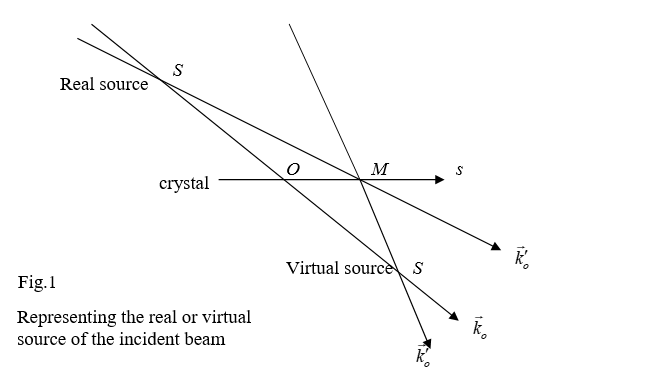
\includegraphics[width=0.95\textwidth]{Fig1.png}
\end{figure}

\begin{figure}
\label{FIG_LENS2}
\caption{Reflected rays in the Bragg (top) and Laue (bottom) case, with a real or virtual focus.}
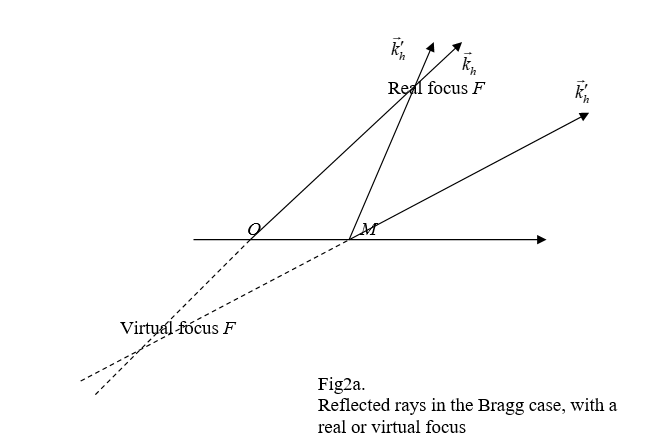
\includegraphics[width=0.49\textwidth]{Fig2a.png}
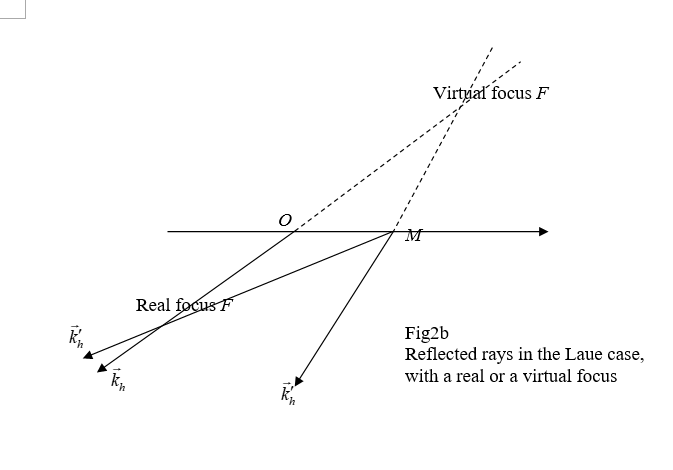
\includegraphics[width=0.49\textwidth]{Fig2b.png}
\end{figure}

The radius of curvature $R$ is set as positive if the X-ray beam is incident on the concave side of the bent crystal surface. The focus distance $L_h$ is set as positive if the real or virtual focus is \inblue{situated on the incidence side on the crystal.} With these conventions, $(\vec n,\vec n')=s/R$, $\epsilon_0 L_0 = s \cos\varphi_0$,  $\epsilon_h L_h = s |\cos\varphi_h|$. Using the relationship
\begin{equation}
    \varphi'_{0,h} = 
    \inred{(\var n', \k'_{0,h})} = 
    (\vec n', \vec n) + (\vec n,\vec k_{0,h}) + (\vec k_{0,h}, \vec{k'_{0,h}}) = -\frac{s}{R} + \varphi_{0,h} + \epsilon_{0,h},
\end{equation}
we obtain

\begin{equation}
\label{angles}
\Delta \varphi_0 = s \frac{\cos\varphi_0}{L_0} - \frac{s}{R}
\end{equation}
and 
\begin{equation}
\Delta \varphi_h = s \frac{|\cos\varphi_h|}{L_h} - \frac{s}{R}.
\end{equation}

The crystal lens equation is finally obtained by inserting these expressions in equation~(\ref{eq:invariant})

\begin{equation}
\label{eq:CLE}
\frac{|\cos\varphi_h| \cos\varphi_0}{L_h} - \frac{\cos^2\varphi_0}{L_0} = \frac{\cos\varphi_h - \cos\varphi_0}{R}.
\end{equation}


Equation~\ref{eq:CLE} is valid in both Bragg and Laue cases. In the Laue symmetrical \inred{PLANE??} case ($\cos\varphi_h=\cos\varphi_0$) it correctly predicts $L_h=L_0$ \inblue{(the focus is at the source, therefore there is no real focus)} and particularly that a plane incident wave produces a plane reflected wave ($L_h$ infinite if $L_0$ is itself infinite).

\inblue{The Crystal Lens equation obtained here (equation~(\ref{eq:CLE})) is different from the equation given in \cite{CK}\footnote{ 
$
\cos\varphi_h |\cos\varphi_0|/L_h + \cos^2\varphi_0/L_0 = (\cos\varphi_0 + \cos\varphi_h)/R 
$}. Both equations are actually equivalent in the Bragg case ($\cos\varphi_h<0$), but not in the Laue case. }

% Formula (\ref{lensequation}) is the correct 'lens equation' valid in both Laue and Bragg cases. In the Laue symmetrical case, for which $\cos\varphi_h=\cos\varphi_0$ , it predicts  $L_h$ infinite if $L_0$ is itself infinite: in other words, a plane incident wave would produce a plane reflected wave. This can be also derived by using simple geometrical arguments in reciprocal space, in the case of an infinitely thin crystal.


\section{Dynamical focusing}

As shown in Ref.~\cite{GuigayFerrero2012}, a double focusing is produced at the following distances from a cylindrically curved crystal, in the symmetric Laue case:

\begin{subequations}
\label{EQ1}
\begin{eqnarray}
{q_1} = R'\frac{{{p_e} - {q_{dyn}}}}{{{p_e} - {q_{dyn}} - R'}} = R'\frac{{{q_{dyn}}(R' + p) - R'p}}{{{q_{dyn}}(R' + p) + {{R'}^2}}} \\
{q_2} = R'\frac{{{p_e} + {q_{dyn}}}}{{{p_e} + {q_{dyn}} - R'}} = R'\frac{{{q_{dyn}}(R' + p) + R'p}}{{{q_{dyn}}(R' + p) - {{R'}^2}}}
\end{eqnarray}
\end{subequations}
$R' = R\cos {\theta _B}$ , the radius $R$ is positive if the incident beam is on the convex side of the bent crystal.  ${p_e} = \frac{{pR'}}{{p + R'}}$, $ p$ is the source-to-crystal distance taken as positive in the case of a real source and negative in the case of a virtual source.  ${q_{1,2}}$  is positive for a real focus and is negative for a virtual focus. Note that  ${q_{1,2}}$ are interchanged when changing the sign of $q_{dyn}$ . By setting $q_{dyn}=0$, we obtain $q_1=q_2=-p$  which results precisely from the corrected form of the 'lens equation' proposed by Chukhovskii and Krisch \cite{CK}; however, the condition  $q_{dyn}=0$ corresponds to the unrealistic case of an infinitely thin crystal. This leads to the assertion  that, in opposition to the Bragg case, the "lens equation" can be misleading and is consequently to be replaced by the above Eqs.~\ref{EQ1} in the Laue case. 


\subsection{Dynamical focusing for a point-source on a flat crystal surface and the expression of  $q_{dyn}$}

In the case of infinite $R$ (flat crystal) and   $p=0$ (point-source on the crystal entrance surface) ,  we obtain from \ref{EQ1} ${q_{1,2}} =  \pm {q_{dyn}}$ and the expression of   $q_{dyn}$ can be obtained as follows.

In this particular case, the reflected amplitude, perpendicularly to the reflected direction is given by the Bessel function $D(\eta ) = {J_0}(Z\sqrt {{a^2} - {\eta ^2}} )$ , where  $Z = k\sqrt {{\chi _h}{\chi _{\bar h}}} /\sin 2{\theta _B}$ , $k = 2\pi /\lambda $  and   $a = t\sin {\theta _B}$; if  the crystal thickness is sufficiently  large for the condition   $Za >  > 1$  to be satisfied, we can use the approximation

\begin{equation}
\label{EQ2}
J_0(Z\sqrt {{a^2} - {\eta ^2}} ) \approx \exp (iZa - i\frac{{Z{\eta ^2}}}{{2a}}) + i\exp ( - iZa + i\frac{{Z{\eta ^2}}}{{2a}})
\end{equation}
in the central region $\left| \eta  \right| <  < a$. Note that the two terms in Eq.~\ref{EQ2} correspond to the two sheets of the dispersion surface of the two-beams dynamical theory. The quadratic terms in the arguments of the exponential functions are similar to the transmission function of a convergent or divergent lens respectively, with the following expression of the focal distance
\begin{equation}
\label{EQ3}
{q_{dyn}} = \frac{{ka}}{{{Z_{re}}}} = \frac{{a\sin 2{\theta _B}}}{{{\mathop{\rm Re}\nolimits} \sqrt {{\chi _h}{\chi _{\bar h}}} }}
\end{equation}

The intensity profile at any distance $q$ from the crystal can be calculated rigorously as 
\begin{equation}
I(x,z) = {(\lambda z)^{ - 1}}{\left| {\int\limits_{ - a}^a {d\eta \exp \{ i\pi {{(x - \eta )}^2}} {{(\lambda z)}^{ - 1}}\} {J_0}(Z\sqrt {{a^2} - {u^2}} )} \right|^2}
\end{equation}

The 'axial intensity profile'  $I(0,z)$  shows a strong maximum for  $z =  \pm {Q_{dyn}}$  somewhat smaller  than
${q_{dyn}}$; this is an aberration effect corresponding to the approximation
\begin{equation}
\sqrt {{a^2} - {\eta ^2}}  = a(1 - \frac{{{\eta ^2}}}{{2{a^2}}} + \frac{{{\eta ^4}}}{{8{a^4}}} + ...) \approx a - \frac{{{\eta ^2}}}{{2a}}
\end{equation}
which has been used in Eq.~\ref{EQ2} .
\begin{equation}
\sqrt {{a^2} - {\eta ^2}}  = a(1 - \frac{{{\eta ^2}}}{{2{a^2}}} + \frac{{{\eta ^4}}}{{8{a^4}}} + ...) \approx a - \frac{{{\eta ^2}}}{{2a}}
\end{equation}

We can use the lens equations Eqs.~\ref{EQ1} with  ${q_{dyn}}$ replaced by the numerically obtained  ${Q_{dyn}}$ which depends on the crystal thickness $t$ but not on the crystal curvature. Note that  ${q_{dyn}}$  is proportional to the crystal thickness t. This is approximately true for ${Q_{dyn}}$. 

\subsection{Exemple  symmetrical Si 111}

 Exemple  symmetrical Si 111, 17 Kev, crystal thickness  $t = 300\mu m$, ${q_{dyn}} = 4480mm$, ${Q_{dyn}} = 3350mm$.


\subsubsection{Particular case of a flat crystal} 
Considering  $R' \to \infty $ in (1), we obtain  ${q_{1,2}} \to  - p \pm {Q_{dyn}}$

\subsubsection{The case of a very distant source and a bent crystal}
In the important case such that  the source distance  $p$ is much larger than  $R'$ and ${{\rm{Q}}_{dyn}}$, Eq.~\ref{EQ1} can be simplified as:
\begin{equation}
{q_1} = R'\frac{{{Q_{dyn}} - R'}}{{{Q_{dyn}}}} ; ~~{q_2} = R'\frac{{{Q_{dyn}} + R'}}{{{Q_{dyn}}}}
\end{equation}
         

According to Eq.~\ref{EQ3}, $q_1$  is negative for  $R' > {Q_{dyn}}$, is equal to 0 for  $R' = {Q_{dyn}}$, reaches a maximum   ${q_{1\max }} = {Q_{dyn}}/4$ for  $R' = {Q_{dyn}}/2$  and decreases as $R'$  gets smaller. 
$q_2$ always decreases as  $R'$ gets smaller; its value is  $2R'$ for  $R' = Q_{dyn}$
It is therefore convenient to scale the value of   $R' $ with respect to the value of  $RQ_{dyn}$.
In the case of the above example, for  $R \approx 1700mm \approx {Q_{dyn}}/2$, we obtain two real focusing distances:  $q_1=$840~mm, $q_2=$2520~mm.

\subsubsection{Case of point source on the entrance surface of a bent crystal}

We obtain from Eq.~\ref{EQ1}
\begin{equation}
{q_1} = \frac{{{Q_{dyn}}R'}}{{{Q_{dyn}} + R'}} {\rm{~~~~or~~~~}} \frac{1}{{{q_1}}} = \frac{1}{{R'}} + \frac{1}{{{Q_{dyn}}}}
\end{equation}

\begin{equation}
{q_2} = \frac{{{Q_{dyn}}R'}}{{{Q_{dyn}} - R'}} {\rm{~~~~or~~~~}}  \frac{1}{{{q_2}}} = \frac{1}{{R'}} - \frac{1}{{{Q_{dyn}}}}
\end{equation}

This consistent with the following expression of the reflected amplitude found by solving the Takagi equations analytically:

\begin{equation}
\label{EQ4}
D(\eta ) = {J_0}(Z\sqrt {{a^2} - {\eta ^2}} )\exp ( - ik\eta \frac{{a + \eta }}{{2R'}})
\end{equation}

\subsubsection{The case of a flat crystal}
In the limit  $R' \to \infty $, we obtain from Eq.~\ref{EQ1}:  $p + {q_1} = {Q_{dyn}}$  and $p + {q_2} =  - {Q_{dyn}}$


\section{Relation with the wave-optical approach in the symmetric Laue case}

In Ref.~\cite{GuigayFerrero2012}, we obtain focusing positions in  $q_{1,2}$ such that   $\frac{1}{{{q_1}}} = \frac{1}{{R'}} + \frac{1}{{{Q_{dyn}} - {p_e}}}$  and  $\frac{1}{{{q_2}}} = \frac{1}{{R'}} - \frac{1}{{{Q_{dyn}} + {p_e}}}$, where  $\frac{1}{{{p_e}}} = \frac{1}{p} + \frac{1}{{R'}}$ 

The limit $a \to 0$  of the integral expression representing the reflected wave for  $q=0$ is
\begin{multline}
D(u) = \int\limits_{u - a}^{u + a} {\frac{{d\tau }}{{\sqrt {i\lambda p} }}} \exp (\frac{{i\pi {\tau ^2}}}{{\lambda p}})\exp (i\pi \frac{{\tau (\tau  + a) - u(u + a)}}{{\lambda R\cos {\theta _B}}}) \times \\
{J_0}(Z\sqrt {{a^2} - {{(u - \tau )}^2}} ) \approx 2a\exp (\frac{{i\pi {u^2}}}{{\lambda p}})\frac{{{J_0}(Za)}}{{\sqrt {i\lambda p} }}\\
\end{multline}
 which corresponds to a virtual focus at  $q_{foc}=-p$, in agreement with the lens equation.
 
Note that this result is obtained by setting ${Q_{dyn}} = 0$  in the general focusing condition which is 
\begin{equation}
{p_e} + {q_e} = R'\frac{{p + q}}{{(p + R')(R' - q)}} = {Q_{dyn}}
\end{equation}


\section{Relation with the wave-optical approach in the general asymmetric Laue case}

Following here the notation of Ref.~\cite{GuigayFerrero2016}, we derive a focusing condition in the limit of vanishing crystal thickness and show its equivalence with the lens equation (7).

The limit   $a \to 0$ of the integral expression representing the reflected wave for  $q=0$ ii:
\begin{equation}
 \exp (\frac{{ik{u^2}}}{{2p}})\exp ( - ik{u^2}\frac{{1 - \gamma }}{{2R\cos {\theta _2}}})
\end{equation}

Following the wave-optical formulation of Ref.~\cite{GuigayFerrero2016}, the lens equation should be  $p_e + q_e = 0$  which can be expressed as
\begin{equation}
\frac{1}{q} + \frac{{{\gamma ^2}}}{p} - \frac{{{\mu _1} + {\gamma ^2}{\mu _2} + 2g}}{R} = 0
\end{equation}
where   $\cos\theta_1 = \gamma \cos\theta_2$,  $\theta_{1,2}=\alpha\pm\theta_B$,

\begin{equation}
{\mu _{1,2}} = \frac{{\sin \alpha ({{\sin }^2}{\theta _{1,2}} + \rho {{\cos }^2}{\theta _{1,2}}) + \cos \alpha \sin 2{\theta _{1,2}}}}{{\sin 2{\theta _B}\cos {\theta _B}}}
\end{equation}
 
\begin{equation}
g =  - \gamma \sin \alpha \frac{{1 + (1 + \rho ){\rm{cos}}{\theta _{\rm{1}}}{\rm{cos}}{\theta _{\rm{2}}}}}{{\cos {\theta _B}\sin 2{\theta _B}}} =  - \sin \alpha \frac{{\gamma  + (1 + \rho ){\rm{co}}{{\rm{s}}^{\rm{2}}}{\theta _{\rm{1}}}}}{{\cos {\theta _B}\sin 2{\theta _B}}}
\end{equation}
 
The parameter $\rho$ is eliminated in 
 
\begin{equation}
{\mu _1} + g = \frac{{\cos \alpha \sin 2{\theta _1} - \sin \alpha (\gamma  + \cos 2{\theta _1})}}{{\cos {\theta _B}\sin 2{\theta _B}}}
\end{equation}

\begin{equation}
{\gamma ^2}{\mu _2} + g = \frac{{{\gamma ^2}\cos \alpha \sin 2{\theta _2} - \sin \alpha (\gamma  + {\gamma ^2}\cos 2{\theta _2})}}{{\cos {\theta _B}\sin 2{\theta _B}}}
\end{equation}

By using the relations

\begin{equation}
\sin 2{\theta _1} + {\gamma ^2}\sin 2{\theta _2} = 2\gamma (\sin {\theta _1}\cos {\theta _2} + \frac{{\cos {\theta _1}}}{{\cos {\theta _2}}}\sin {\theta _2}\cos {\theta _2}) = 2\gamma \sin ({\theta _1} + {\theta _2}) = 2\gamma \sin 2\alpha 
\end{equation}
and $\sin 2\alpha \cos \alpha  - \sin \alpha  = \sin \alpha (2{\cos ^2}\alpha  - 1) = \sin \alpha \cos 2\alpha $
we can write

\begin{equation}
{\mu _1} + {\gamma ^2}{\mu _2} + 2g = \frac{{2\gamma \sin 2\alpha \cos \alpha  - \sin \alpha (2\gamma  + \cos 2{\theta _1} + {\gamma ^2}\cos 2{\theta _2})}}{{\cos {\theta _B}\sin 2{\theta _B}}} = \sin \alpha \frac{{2\gamma \cos 2\alpha  - \cos 2{\theta _1} - {\gamma ^2}\cos 2{\theta _2}}}{{\cos {\theta _B}\sin 2{\theta _B}}}
\end{equation}

This last expression will be written in a simpler form as follows. Using 
\begin{equation}
\begin{array}{l}
\cos 2{\theta _1} + {\gamma ^2}\cos 2{\theta _2} = 2{\cos ^2}{\theta _1} - 1 + 2{\gamma ^2}{\cos ^2}{\theta _2} - {\gamma ^2} = 4{\cos ^2}{\theta _1} - 1 - {\gamma ^2} = 4\gamma \cos {\theta _1}\cos {\theta _2} - 1 - {\gamma ^2}\\
{\rm{   }} = 2\gamma [\cos ({\theta _1} + {\theta _2}) + \cos ({\theta _1} - {\theta _2})] - 1 - {\gamma ^2} = 2\gamma [\cos 2\alpha  + \cos 2{\theta _B}] - 1 - {\gamma ^2}
\end{array}
\end{equation}

we obtain 
\begin{equation}
2\gamma \cos 2\alpha  - \cos 2{\theta _1} - {\gamma ^2}\cos 2{\theta _2} = 1 + {\gamma ^2} - 2\gamma \cos 2{\theta _B} = \frac{{{{\cos }^2}{\theta _2} + {{\cos }^2}{\theta _1} - 2\cos {\theta _1}\cos {\theta _2}\cos 2{\theta _B}}}{{{{\cos }^2}{\theta _2}}}
\end{equation}
 by using
 \begin{equation}
 \begin{array}{l}
{\cos ^2}{\theta _2} + {\cos ^2}{\theta _1} - 2\cos {\theta _1}\cos {\theta _2}\cos 2{\theta _B} = \frac{{1 + \cos 2{\theta _1}}}{2} + \frac{{1 + \cos 2{\theta _2}}}{2} - [\cos ({\theta _1} + {\theta _2}) + \cos ({\theta _1} - {\theta _2})]\cos 2{\theta _B}\\
{\rm{   }} = \frac{{2 + \cos (2\alpha  + 2{\theta _B}) + \cos (2\alpha  - 2{\theta _B})}}{2} - [\cos 2\alpha  + \cos 2{\theta _B}]\cos 2{\theta _B}\\
{\rm{      }} = 1 + \cos 2\alpha \cos 2{\theta _B} - [\cos 2\alpha  + \cos 2{\theta _B}]\cos 2{\theta _B} = {\sin ^2}2{\theta _B}
\end{array}
\end{equation}

and also 
\begin{equation}
\cos {\theta _2} - \cos {\theta _1} = \cos (\alpha  - {\theta _B}) - \cos (\alpha  + {\theta _B}) = 2\sin \alpha \sin {\theta _B} = (1 - \gamma )\cos {\theta _2}
\end{equation}
we finally obtain 
\begin{equation}
{\mu _1} + {\gamma ^2}{\mu _2} + 2g = \sin \alpha \frac{{2\sin {\theta _B}}}{{{{\cos }^2}{\theta _2}}} = \frac{{(1 - \gamma )\cos {\theta _2}}}{{2\sin {\theta _B}}}\frac{{2\sin {\theta _B}}}{{{{\cos }^2}{\theta _2}}} = \frac{{1 - \gamma }}{{\cos {\theta _2}}}
\end{equation}

Equation (8) is therefore:
\begin{equation}
\frac{1}{q} + \frac{{{\gamma ^2}}}{p} = \frac{{1 - \gamma }}{{R\cos {\theta _2}}}
\end{equation}
which is  
\begin{equation}
\frac{{{{\cos }^2}{\theta _2}}}{q} + \frac{{{{\cos }^2}{\theta _1}}}{p} = \frac{{\cos {\theta _2} - \cos {\theta _1}}}{R}
\end{equation}

We see that this is agreement with  (7), by noting that  $\theta_1=\varphi_0$ , $\theta_2=\varphi_h$ , $\cos\varphi_h>0$ , $q=-L_h$  and that the radius of curvature  $R$  is to be inversed, because $R$ is taken as positive for beam incidence on the convex side of the crystal in Ref.~\cite{GuigayFerrero2016}.

\subsection{Demonstration of (8) :}

\begin{equation}
D(u) = \int\limits_{\gamma (u - a)}^{\gamma (u + a)} {\frac{{d\tau }}{{\sqrt {i\lambda p} }}} \exp (\frac{{i\pi {\tau ^2}}}{{\lambda p}})\exp [i\phi (u,\tau )]M(i\beta ,1,iA({s_o} - {\sigma _o})({s_h} - {\sigma _h}))\\
{\rm{       }}
\end{equation}

\begin{equation}
a = \frac{{t\sin 2{\theta _B}}}{{2\cos {\theta _1}}}
\end{equation}
\begin{equation}
{s_o} = \frac{{a + u}}{{\sin 2{\theta _B}}}
\end{equation}
\begin{equation}
{s_h} = \gamma \frac{{a - u}}{{\sin 2{\theta _B}}}
\end{equation}
\begin{equation}
{\sigma _o} = \frac{\tau }{{\gamma \sin 2{\theta _B}}}
\end{equation}
\begin{equation}
{\sigma _h} = \frac{{ - \tau }}{{\sin 2{\theta _B}}}
\end{equation}

\begin{equation}
A =  - \frac{{2k\sin {\theta _B}}}{R}\sin \alpha [1 + (1 + \rho )\cos {\theta _1}\cos {\theta _2}]
\end{equation}
\begin{equation}
g = \frac{{A\gamma R}}{{k{{\sin }^2}2{\theta _B}}}
\end{equation}


\begin{multline}
\phi (u,\tau ) = {\varphi _2}({\sigma _h}) - {\varphi _1}({s_o}) + A{s_o}{\sigma _h}\\
{\rm{     }} = \frac{k}{{2R}}[ - {\mu _2}\sigma _h^2{\sin ^2}2{\theta _B} + {a_2}{\sigma _h}\sin {\theta _B} - ({\mu _1}s_o^2{\sin ^2}2{\theta _B} - {a_1}{s_o}\sin {\theta _B})] - A\tau \frac{{a + u}}{{{{\sin }^2}2{\theta _B}}}\\
{\rm{    }} = \frac{{ - k}}{{2R}}[{\mu _2}{\tau ^2} + {a_2}\tau  + {\mu _1}{(a + u)^2} - {a_1}(a + u)] - \frac{{kg}}{{\gamma R}}\tau (a + u)\\
 \to \frac{{ - k}}{{2R}}[{\mu _2}{\gamma ^2}{u^2} + {a_2}\gamma u + {\mu _1}{(a + u)^2} - {a_1}(a + u)] - \frac{{kg}}{R}u(a + u){\rm{  as }}\tau  \to \gamma u
\end{multline}

\begin{equation}
({s_o} - {\sigma _o})({s_h} - {\sigma _h}) = \gamma \frac{{(a + u - \tau /\gamma )(a - u + \tau /\gamma )}}{{{{\sin }^2}2{\theta _B}}} \to \frac{{\gamma {a^2}}}{{{{\sin }^2}2{\theta _B}}}
\end{equation}
as   $\tau  \to \gamma u$
where 
\begin{equation}
{a_{1,2}} = t\frac{{\cos \alpha \sin {\theta _{1,2}} + \rho \sin \alpha \cos {\theta _{1,2}}}}{{\cos {\theta _B}}}
\end{equation}

When the crystal thickness goes to 0, the Bragg reflected amplitude is obtained by multiplying the amplitude of the incident beam by the function  $2a\exp ( - ik{u^2}\frac{{1 - \gamma }}{{2R\cos {\theta _2}}})$ . 

Note it can be shown that   
\begin{equation}
 {a_2}\gamma  + 2{\mu _1}a - {a_1} + 2ga = t\tan {\theta _B}\frac{{{{\cos }^2}{\theta _B} - {{\sin }^2}\alpha  - {{\cos }^2}{\theta _1}}}{{\cos {\theta _2}\cos {\theta _1}}},m
\end{equation}


\section{Polychromatic focusing}

As pointed out by Chukhovski and Krisch in Ref.~\cite{CK}, the monochromatic focusing is not to be confused with the polychromatic formula (ref..), in which the X-ray energy of the incident rays is varied in order to satisfy locally the exact Bragg condition. The Bragg angle is varied, whereas the asymmetry angle is constant. Then, according to (1),   ${\varphi _o} + {\varphi _h}$  is constant . We thus have  $\Delta {\varphi _o} + \Delta {\varphi _h} = 0$ , with  $\Delta {\varphi _o} = s\frac{{\cos {\varphi _o}}}{{{L_o}}} - \frac{s}{R}$  and $\Delta {\varphi _h} = s\frac{{\left| {\cos {\varphi _h}} \right|}}{{{L_h}}} - \frac{s}{R}$ .

The polychromatic formula is therefore:
\begin{equation}
\frac{{\cos {\varphi _o}}}{{{L_o}}} + \frac{{\left| {\cos {\varphi _h}} \right|}}{{{L_h}}} = \frac{2}{R}
\end{equation}

This polychromatic formula coincide with (4) in the symmetric Bragg case (not in symmetric Laue case.

\subsection{Rowland condition}

This implies  ${L_o} = R\cos {\varphi _o}$ ,  ${L_h} = R\left| {\cos {\varphi _h}} \right|$
Both equations (4) and (5) are then satisfied.


\section{Discussion and examples}

ojfds

\section{Summary and conclusions}

%
%%%%%%%%%%%%%%%%%%%%%%%%%%%%%%%%%%%%%%%%%%%%%%%%%%%%%%%%%%%%%%%%%%%%%%%%%%%%%%%%%%%%%%%%%%%%%%%%%%%%%%%%%%%%%%%%%%%%%%%%%%%%%%%%%%%%%%%%%%%%%%%%%%%%%%%%%
%
\ack{Acknowledgements}
A large part of this work comes from ...


\bibliography{iucr} % reads iucr.bib with items
\bibliographystyle{iucr}
%\referencelist{library}

%\appendix
%\section{Fourier Transform and FFT}


     %-------------------------------------------------------------------------
     % The back matter of the paper - acknowledgements and references
     %-------------------------------------------------------------------------

     % Acknowledgements come after the appendices



     % References are at the end of the document, between \begin{references}
     % and \end{references} tags. Each reference is in a \reference entry.

%\begin{references}
%\reference{Author, A. \& Author, B. (1984). \emph{Journal} \textbf{Vol}, first page--last page.}
%\end{references}
%\cite{knuth84}

%\begin{thebibliography}{30}
%\expandafter\ifx\csname natexlab\endcsname\relax\def\natexlab#1{#1}\fi
%\expandafter\ifx\csname bibnamefont\endcsname\relax
%  \def\bibnamefont#1{#1}\fi
%\expandafter\ifx\csname bibfnamefont\endcsname\relax
%  \def\bibfnamefont#1{#1}\fi
%\expandafter\ifx\csname citenamefont\endcsname\relax
%  \def\citenamefont#1{#1}\fi
%\expandafter\ifx\csname url\endcsname\relax
%  \def\url#1{\texttt{#1}}\fi
%\expandafter\ifx\csname urlprefix\endcsname\relax\def\urlprefix{URL }\fi
%\providecommand{\bibinfo}[2]{#2}
%\providecommand{\eprint}[2][]{\url{#2}}
%
%\bibitem[{\citenamefont{Shvyd'ko}(2016)}]{GuigayFerrero2012}
%\bibinfo{author}{\bibfnamefont{Yu.}~\bibnamefont{Shvyd'ko}},
%\bibinfo{journal}{Phys. Rev. Lett.} \textbf{\bibinfo{volume}{116}},
%\bibinfo{pages}{080801} (\bibinfo{year}{2016}).
%
%%\bibitem[{\citenamefont{Guigay and Ferrero}]{ddd}
%%\bibinfo{author}{\bibfnamefont{Jean-Pierre}~\bibnamefont{Guigay}},
%%\bibinfo{author}{\bibfnamefont{Claudio}~\bibnamefont{Ferrero}},
% % \bibinfo{journal}{xxxx} \textbf{\bibinfo{volume}{xx}},
% % \bibinfo{pages}{xx} (\bibinfo{year}{2012}).
%
%\end{thebibliography}

%% Note added by Overleaf: If using bibtex, remove the "references" environment above, and uncomment the following lines.

%\bibliographystyle{iucr}
%\referencelist{iucr}

%      %-------------------------------------------------------------------------
%      % TABLES AND FIGURES SHOULD BE INSERTED AFTER THE MAIN BODY OF THE TEXT
%      %-------------------------------------------------------------------------
% 
%      % Simple tables should use the tabular environment according to this
%      % model
% 
% \begin{table}
% \caption{Caption to table}
% \begin{tabular}{llcr}      % Alignment for each cell: l=left, c=center, r=right
%  HEADING    & FOR        & EACH       & COLUMN     \\
% \hline
%  entry      & entry      & entry      & entry      \\
%  entry      & entry      & entry      & entry      \\
%  entry      & entry      & entry      & entry      \\
% \end{tabular}
% \end{table}
% 
%      % Postscript figures can be included with multiple figure blocks
% 
% \begin{figure}
% \caption{Caption describing figure.}
% 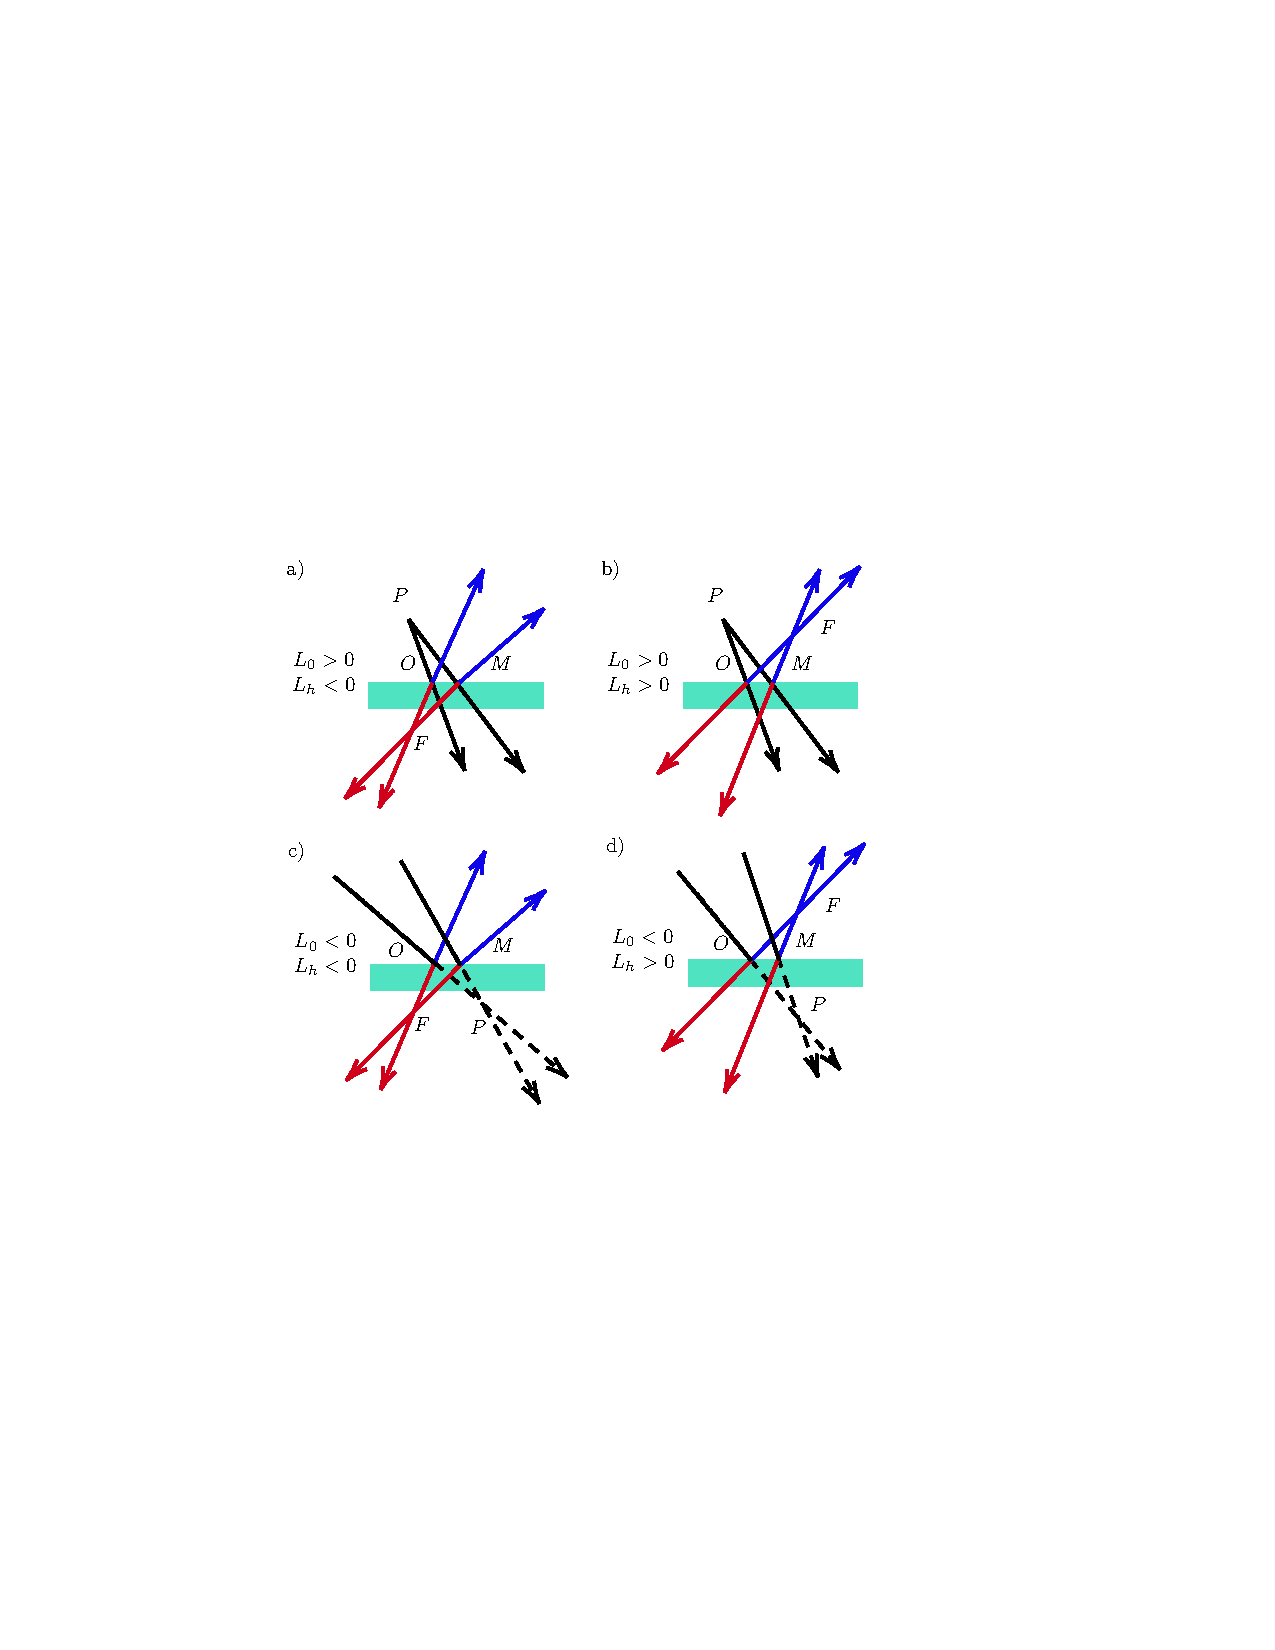
\includegraphics{fig1}
% \end{figure}


\end{document}                    % DO NOT DELETE THIS LINE
%%%%%%%%%%%%%%%%%%%%%%%%%%%%%%%%%%%%%%%%%%%%%%%%%%%%%%%%%%%%%%%%%%%%%%%%%%%%%%
